\documentclass[adobefonts, nocap]{ctexart}
\usepackage{amsmath}
\usepackage{amsfonts}
\usepackage{listings}
\usepackage{xcolor}
\usepackage{graphicx}
\usepackage{siunitx}
\usepackage{hyperref}
\hypersetup{
  colorlinks = true,
  linkcolor = blue,
  unicode = true
}
\lstset{
  language = C,
  basicstyle = \small\ttfamily,
  keywordstyle = \small\ttfamily\color{red},
  stringstyle = \color{gray},
  numbers = left,
  numberstyle = \small,
  numbersep = 5pt,
  frame = leftline,
  showstringspaces = false
}
\def\D{\mathrm{d}}
\begin{document}
  \title{计算机系统结构第六次作业}
  \author{李雨田\hspace{1em}2010012193\hspace{1em}计14}
  \maketitle
  \section*{9.9}
    \subsection*{(1)}
      \[
        Cube_{2}(12)=Cube_{2}(01100_{2})=01000_{2}=8.
      \]
      \[
        \sigma(8)=\sigma(01000_{2})=10000_{2}=16.
      \]
      \[
        \beta(9)=\beta(01001_{2})=11000_{2}=24.
      \]
      \[
        PM2_{+3}(28)=PM2_{+3}(11100_{2})=00100_{2}=4.
      \]
      \[
        Cube_{0}(\sigma(4))=Cube_{0}(\sigma(00100_{2}))=Cube_{0}(01000_{2})=01001_{9}=9.
      \]
      \[
        \sigma(Cube_{0}(18))=\sigma(Cube_{0}(10010_{2}))=\sigma(10011_{2})=00111_{2}=7.
      \]
    \subsection*{(2)}
      用$Cube_{0}$和$\sigma$构成混洗交换网中,只有循环位移和修改最低位两种操作.要从$00000$到$11111$,需要进行$5$次$\sigma$操作和$4$次$Cube_{0}$操作.网络直径是$9$.

      $5$号机为$00101_{2}$, $7$号机为$00111_{2}$.要经过
      \[
        00101_{2}\rightarrow 00100_{2}\rightarrow 01000_{2}\rightarrow 01001_{2}\rightarrow 10010_{2}\rightarrow 10011_{2}\rightarrow 00111_{2}.
      \]

      一共$6$步.
    \subsection*{(3)}
      采用移数网络构成互连网,此时$n=5$,节点度为$9$,直径为$3$.距离$2$号机最远的是$13$, $15$, $21$, $23$号处理机.
  \section*{9.13}
    如下图所示.

    \begin{center}
      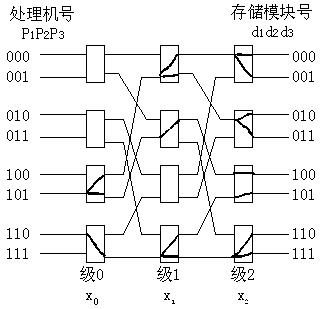
\includegraphics[width=10cm]{1.png}
    \end{center}
\end{document}
